% Clase del documento (class)
\documentclass[a4paper,12pt]{article}
%\documentclass[a4paper,10pt]{scrartcl}

%-------------------------------------------------------------------------------
% Preámbulo del documento (preamble)
% Paquetes incluidos
%\usepackage[latin1]{inputenc}
\usepackage[utf8]{inputenc}
\usepackage[T1]{fontenc}
\usepackage[spanish]{babel}
\usepackage{graphicx}
\usepackage[nottoc, notlot, notlof, notindex]{tocbibind}	% Incluye la bibliografía (referencias) en el índice (tabla de contenidos).
% Las opciones son:
% notoc -> no incluir el índice general
% notlot -> no incluir el índice de tablas
% notlof -> no incluir el índice de figuras
% notindex -> no incluir el índice alfabético
% notbib -> no incluir la bibliografía


% Formato de los márgenes
\usepackage{anysize}
\marginsize{2.5cm}{2.5cm}{2.5cm}{2.5cm}

% Título, autor, fecha, etc.
\title{Pronóstico de Partidos de Fútbol:\\Manual de Usuario}
\author{José Miguel Horcas Aguilera}
\date{2/06/2010}

% Información para el pdf.
\pdfinfo{%
  /Title    ()
  /Author   ()
  /Creator  ()
  /Producer ()
  /Subject  ()
  /Keywords ()
}

%---------------------------------------------------------------------------------
% Cuerpo del documento (document body)
\begin{document}
%\renewcommand{\labelitemi}{$\bullet$ }
\renewcommand{\figurename}{Figura}
\maketitle
\tableofcontents
\newpage

\section{Descripción}
\label{sec:Descripción}
La aplicación nos permite predecir el resultado de un partido de fútbol,
informándonos de las probabilidades para los diferentes resultados posibles, el signo (1, X ó 2) del partido y las probabilidades que tiene cada equipo de marcar un número determinado de goles.
El programa nos pedirá la información necesaria a través de un formulario en el cuál se irán respondiendo diferentes preguntas relacionadas con el partido de fútbol y los equipos enfrentados.
\section{Instalación}
\label{sec:instalacion}
\par
Para ejecutar correctamente el programa es necesario que los ficheros
\textit{pronosticoFutbol.jar}, \textit{redFutbol.xdsl} y \textit{smile.jar} se encuentren en el mismo directorio.\footnote{¡Atención!: no cambiar el nombre de los ficheros \textit{redFutbol.xdsl} y \textit{smile.jar}, sino el programa no los reconocerá.}

\subsection{Requisitos mínimos}
Los requisitos mínimos para la ejecución del programa son:
\begin{itemize}
  \item Tener instalada la Máquina Virtual de Java (JVM).\\
	Se puede obtener gratuitamente en: \texttt{http://www.java.com/es/download/index.jsp}
  \item Colocar la biblioteca jsmile propia del sistema operativo en el \textit{ClassPath} de Java.
	En la carpeta \textit{BibliotecasJSMILE} incluida con la aplicación se encuentran las bibliotecas necesarias para los diferentes sistemas operativos.
	\begin{itemize}
	 \item Windows:\\
	  Copiar el fichero \textit{smile.dll} en una carpeta y añadir la biblioteca al path.
	  Para añadirla al path hay que seguir la siguiente secuencia de pasos:
	  (suponiendo que la hemos copiado en \texttt{C:\textbackslash lib\textbackslash win32})
		\begin{enumerate}
		 \item Picar con el botón derecho sobre MiPC y en Propiedades, y a continuación seleccionar la pestaña Opciones avanzadas.
		 \item Seleccionar el botón Variables de entorno. En la sección de variables del sistema seleccionar la variable Path.
		 \item Pulsando sobre el botón modificar pasamos a introducir la ruta del directorio donde se encuentra jsmile.dll, en nuestro caso \texttt{C:\textbackslash lib\textbackslash win32}. Finalmente pulsar en aceptar.
		\end{enumerate}
	 \item Linux:\\
	  Copiar el fichero \textit{libjsmile.so} en la ruta:\\ \texttt{/usr/lib/jvm/java-6-sun-VERSION/jre/lib/ARQUITECTURA/}\\

	  donde VERSION es la versión de Java instalada, por ejemplo 1.6.0.20, y ARQUITECTURA es la arquitectura del ordenador (i386, amd64, ...).		
	 \item MacOSX:\\
	  Copiar el fichero \textit{libjsmile.jnilib} en el directorio:\\ \texttt{/Sistema/Librería/Frameworks/JavaVM.framework/Versions/1.6.0/Libraries}

	\end{itemize}
\end{itemize}

\section{Ejecución}
El programa se puede ejecutar simplemente haciendo doble clic sobre el fichero \textit{PronosticoFutbol.jar}.
Aunque también es posible ejecutarlo desde un terminal de línea de comandos con la siguiente instrucción:
\texttt{java -jar PronosticoFutbol.jar}

%\clearpage
\section{Funcionamiento}
Tanto el aspecto de la aplicación como su funcionamiento son fáciles de entender. 
El programa sólo dispone de una pantalla principal dividida en cuatro pestañas como se puede ver en la figura~\ref{fig:pestaña1}.
\begin{figure}[h]
 \begin{center}
  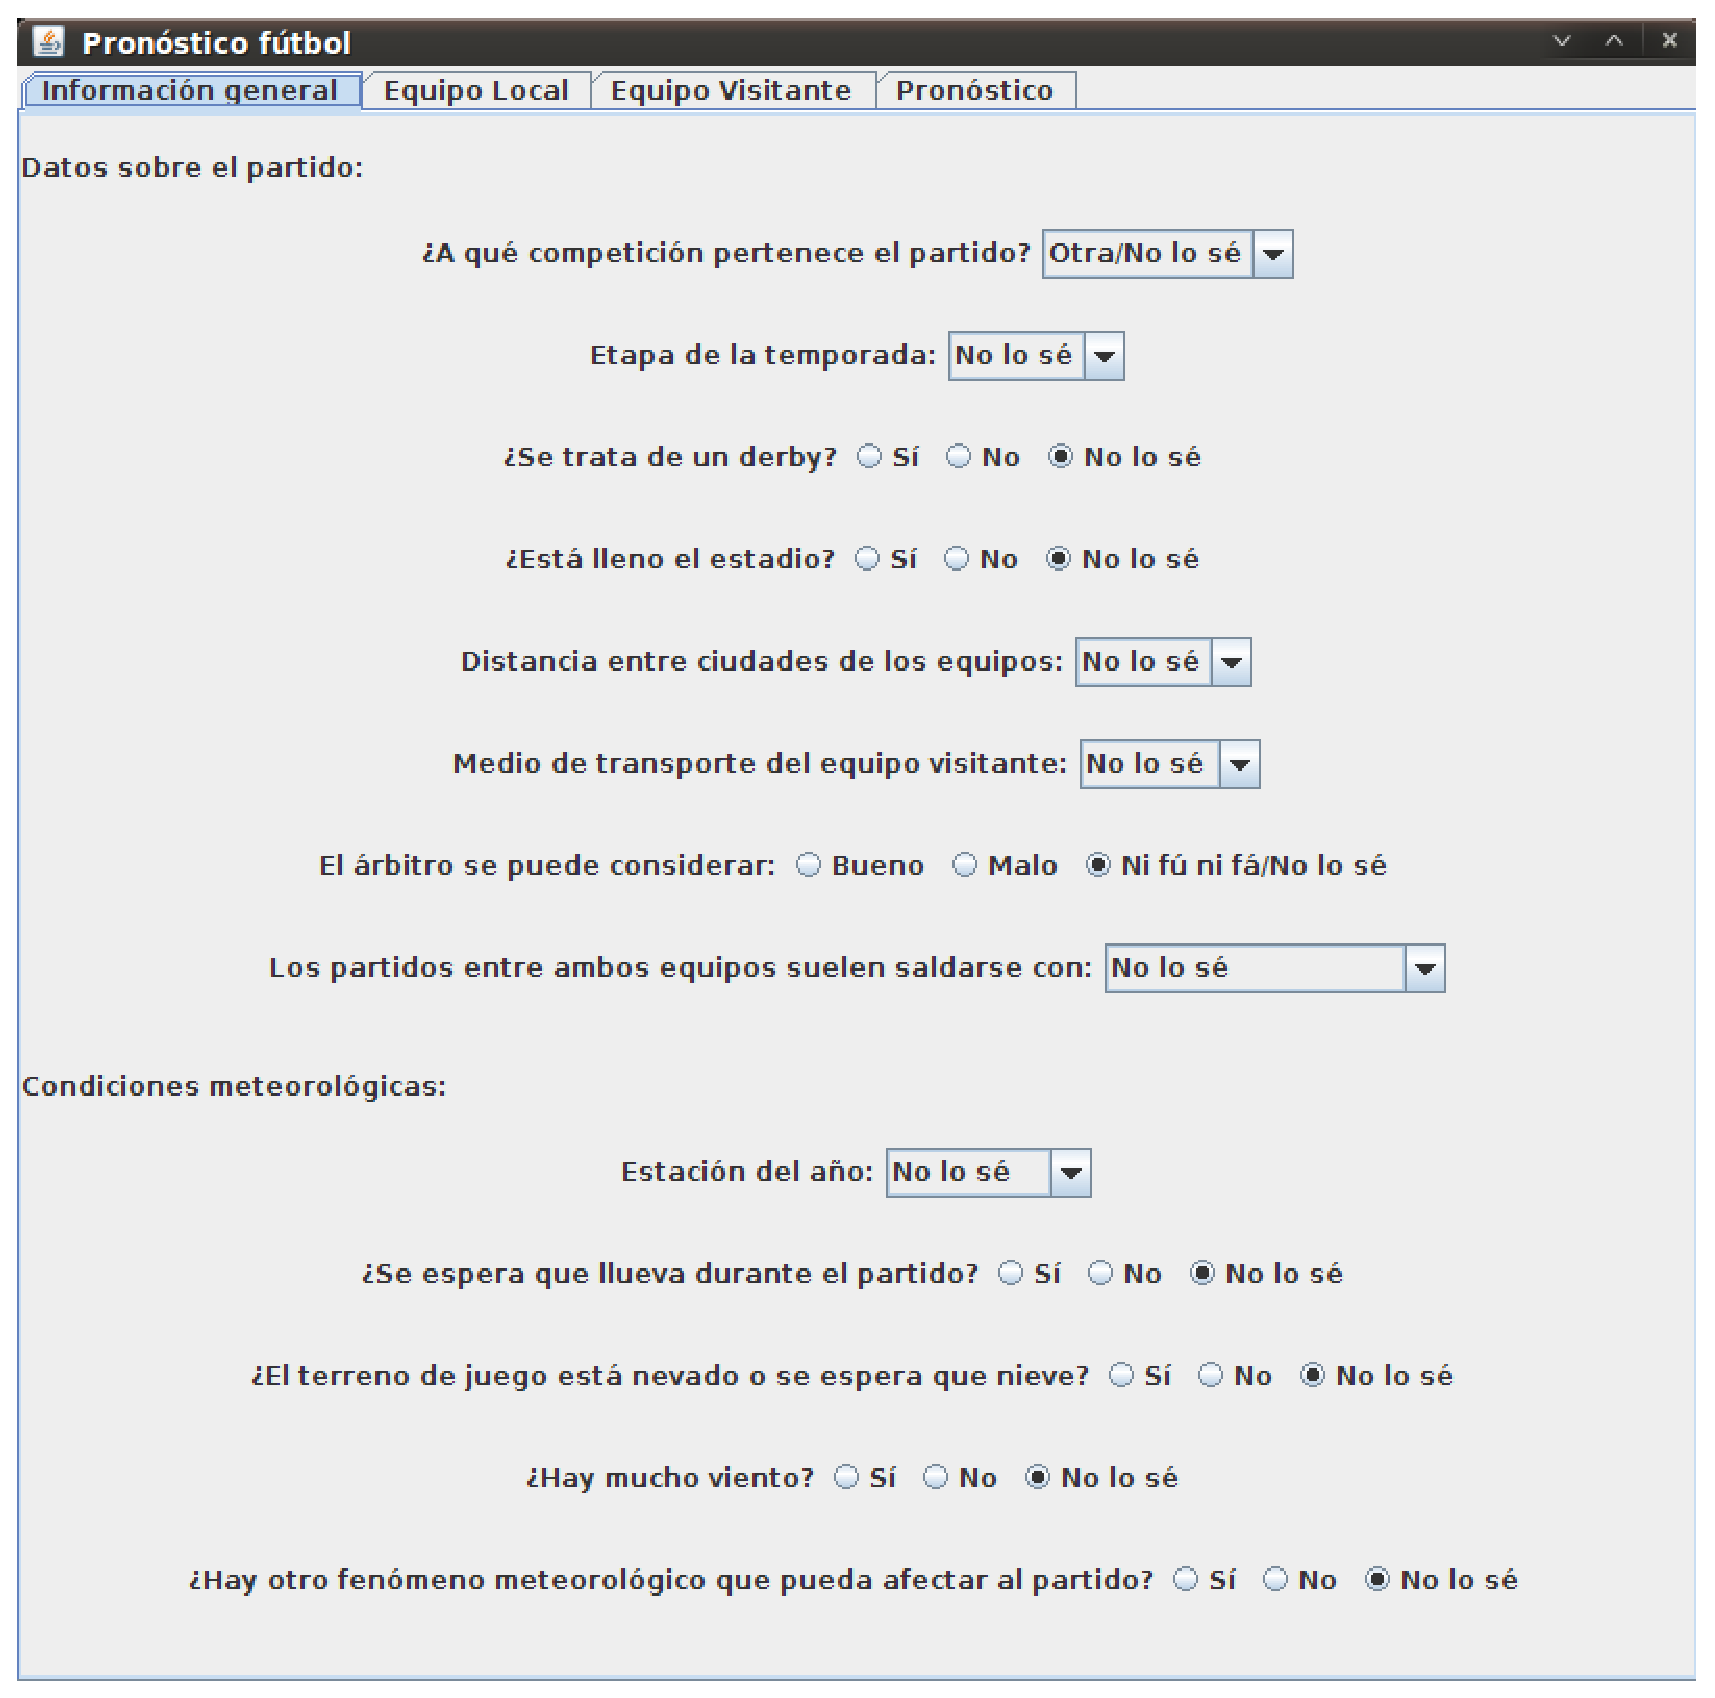
\includegraphics[scale=0.4]{p1.eps}
\caption{Pantalla principal del programa con la primera pestaña activada.}
\label{fig:pestaña1}
 \end{center}
\end{figure} 

Las tres primeras pestañas son las encargadas de recoger los datos proporcionados por el usuario, mientras que la última pestaña muestra los resultados.
\\
Nótese que pueden realizarse todos los cambios que se deseen sobre la información cada vez que se necesite,
los resultados se actualizarán automáticamente cada vez que se active la última pestaña.

\subsection{Introduciendo los datos}
La forma de preguntar los datos al usuario se hace de manera variada dependiendo del tipo de información.

\begin{itemize}
 \item Para datos numéricos el programa ofrece un recuadro como el de la figura~\ref{fig:campoNumerico} en el cuál el usuario debe introducir los valores.
  En caso de introducir un valor no válido el programa ignorará esa entrada igual que si se dejara sin rellenar.
\begin{figure}[h]
 \begin{center}
  
\includegraphics[scale=0.8]{numerico.eps}
\caption{Campo para introducir valores numéricos.}
\label{fig:campoNumerico}
 \end{center}
\end{figure} 

 \item Otros datos pueden ser proporcionados mediante listas desplegables (figura~\ref{fig:listaDesplegable}) en la cuales se eligirá una de las posibles opciones.
\begin{figure}[h]
 \begin{center}
  
\includegraphics[scale=0.8]{listaDesplegable.eps}
\caption{Lista desplegable que nos muestra las posibles opciones.}
\label{fig:listaDesplegable}
 \end{center}
\end{figure} 

 \item La mayoría de los datos se introducirán mediante la elección de una casilla a elegir entre varias, como el mostrado en la figura~\ref{fig:check}.
\begin{figure}[h]
 \begin{center}
  
\includegraphics[scale=0.8]{check.eps}
\caption{Diferentes opciones a elegir para introducir un dato.}
\label{fig:check}
 \end{center}
\end{figure} 

\end{itemize}

En todos los casos se encuentra activada la opción por defecto para la situación en la que el usuario no conozca el dato pedido o no disponga de la información necesaria.
El programa tendrá esto en cuenta, y aun así nos dará un pronóstico para el partido.
\\\par
A continuación se describe el contenido de las diferentes pestañas.

\subsubsection{Información general}
La primera pestaña \textit{Información general}, que se encuentra activada por defecto, nos ofrece la posibilidad de introducir datos generales sobre el partido.
Estos datos serán desde la competición a la que pertenece el partido (liga, amistoso,...) hasta las condiciones meteorológicas que puedan afectar al desarrollo del mismo.

\subsubsection{Equipo Local}
La segunda pestaña \textit{Equipo Local} muestra otra tanda de preguntas; en este caso se trata de datos concretos sobre el equipo local,
desde el presupuesto del equipo o el número de jugadores de la plantilla hasta datos históricos como los goles por partido que suele marcar o el número de títulos ganados.
En la figura~\ref{fig:p2} puede verse la apariencia de esta pestaña.
\begin{figure}[h]
 \begin{center}
  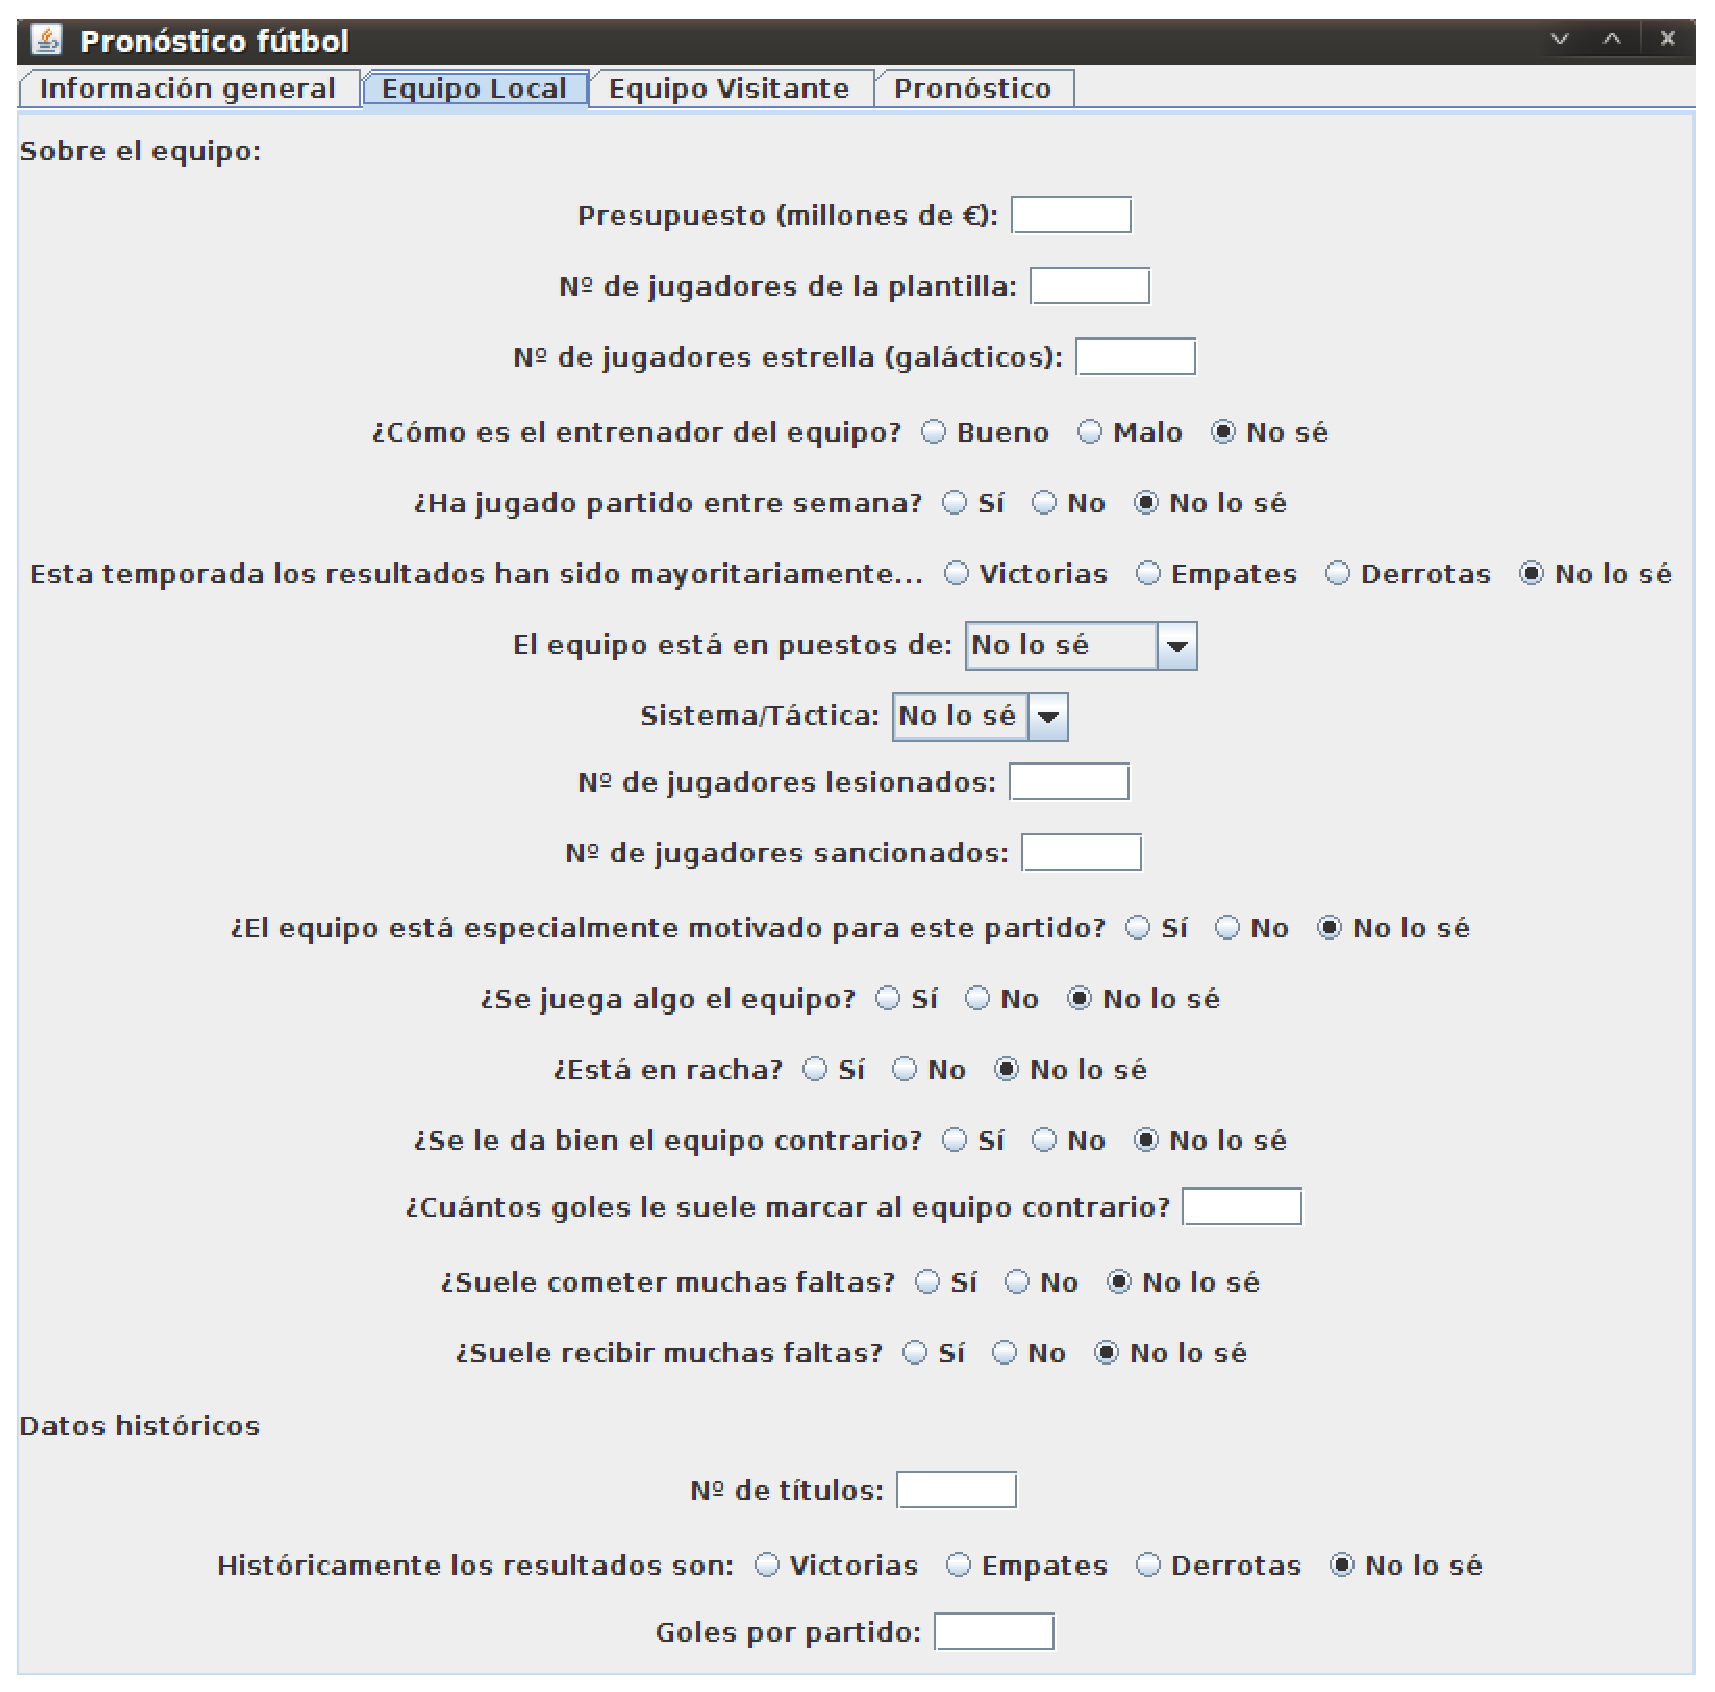
\includegraphics[scale=0.4]{p2.eps}
\caption{Pestaña para introducir la información del equipo local.}
\label{fig:p2}
 \end{center}
\end{figure} 

\subsubsection{Equipo Visitante}
La tercera pestaña \textit{Equipo Visitante} es idéntica a la pestaña anterior, pero los datos serán relativos al equipo visitante.

\subsection{Visualizando los resultados}
El programa presenta los resultados de una manera cómoda para el usuario a través de la última pestaña.
Los resultados se actualizan automáticamente cada vez que se activa esta pestaña. 
La figura~\ref{fig:p4} muestra su aspecto.
\begin{figure}[h]
 \begin{center}
  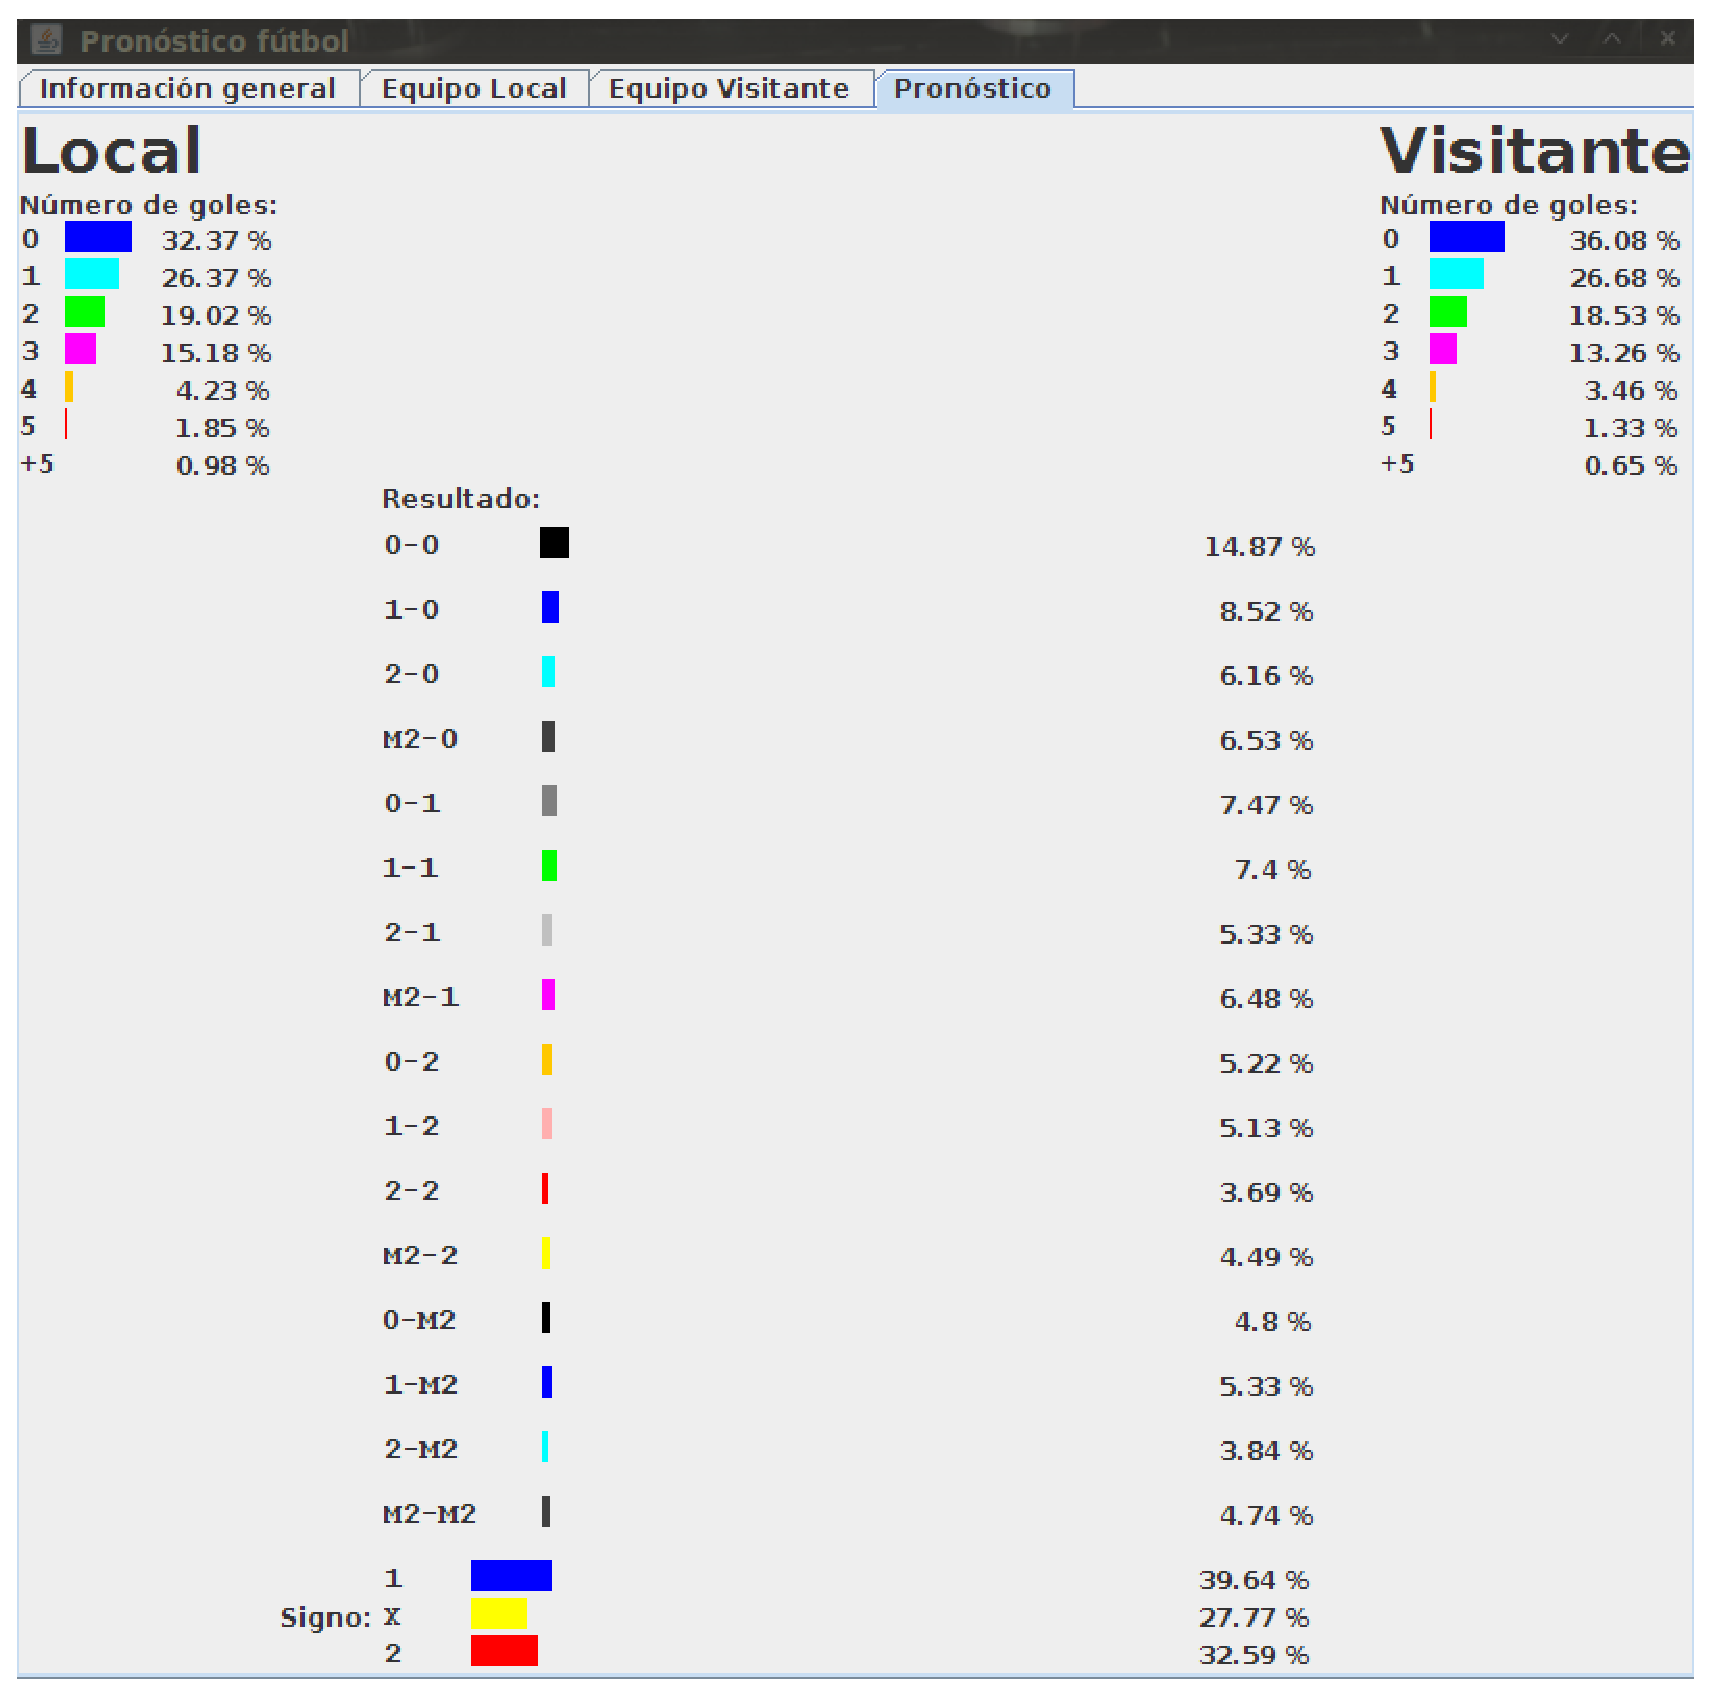
\includegraphics[scale=0.4]{p4.eps}
\caption{Pestaña con los resultados del pronóstico.}
\label{fig:p4}
 \end{center}
\end{figure} 

\subsubsection{Pronóstico}
La pestaña \textit{Pronóstico} muestra las probabilidades de cada equipo (a la izquierda el equipo local y a la derecha el equipo visitante)
del número de goles que marcará en este partido.
En el centro de la pantalla aparecen las probabilidades para los diferentes resultados del partido, donde M2 indica más de dos goles.
Y en la parte inferior aparecen las probabilidades del signo del partido, esto es, 1, X ó 2 en función de si gana el equipo local, hay empate, o gana el equipo visitante respectivamente.
Las probabilidades se indican de dos formas (figura~\ref{fig:goles}): una mediante barras de colores, y otra mostrando el porcentaje a la derecha de cada barra.
\begin{figure}[h]
 \begin{center}
  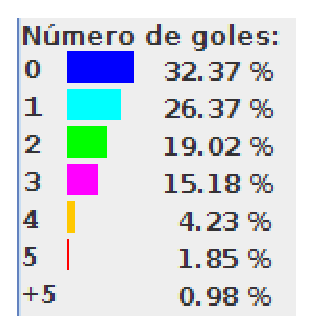
\includegraphics[scale=0.5]{goles.eps}
\caption{Representación de las probabilidades.}
\label{fig:goles}
 \end{center}
\end{figure} 

\section{Obteniendo la información necesaria}
Algunos usuarios pueden encontrar dificultades a la hora de proporcionar algunos datos requeridos por el programa;
sobre todo datos muy específicos de cada equipo, como el presupuesto o el número de goles que le suele marcar al equipo contrario.
Estos datos y muchos más se pueden encontrar fácilmente en guías o anuarios de fútbol que publican todos los años los principales diarios deportivos, como por ejemplo en \cite{GM0910}.
Además, en las páginas webs de dichos diarios (\cite{WEBM}, \cite{WEBAS}) se puede consultar todo tipo de datos estadísticos que pueden ser de utilidad para el programa.

\begin{thebibliography}{10}
\bibitem[GM0910]{GM0910} MARCA. \emph{Guía de la Liga 2010}. Nº 15, Agosto 2009.
\bibitem[WEBM]{WEBM} Sitio oficial del diario deportivo MARCA.\\
  \texttt{http://www.marca.com/}
\bibitem[WEBAS]{WEBAS} Sitio oficial del diario deportivo AS.\\
  \texttt{http://www.as.com/}
\end{thebibliography}

\end{document}
